\documentclass{article}
% Change "article" to "report" to get rid of page number on title page
\usepackage{amsmath,amsfonts,amsthm,amssymb}
\usepackage[all]{xy}
\usepackage{enumerate,verbatim}
\usepackage{setspace}
\usepackage{Tabbing}
\usepackage{fancyhdr}
\usepackage{lastpage}
\usepackage{extramarks}
\usepackage{chngpage}
\usepackage{soul,color}
\usepackage{graphicx,float,wrapfig}
\usepackage{listings}
\usepackage{pdfpages}
\usepackage{graphicx}
\usepackage{epstopdf}
\graphicspath{ {desktop/OpTixGroup/FirstProject} }






% In case you need to adjust margins:
\topmargin=-0.45in      %
\evensidemargin=0in     %
\oddsidemargin=0in      %
\textwidth=6.5in        %
\textheight=9.0in       %
\headsep=0.25in         %

% Homework Specific Information
\newcommand{\hmwkTitle}{Machine Learning Techniques for Film Analysis}
\newcommand{\hmwkClass}{OpTix Group}
\newcommand{\hmwkClassInstructor}{Dutta}
\newcommand{\hmwkAuthorName}{Andrew Dong}

% Setup the header and footer
\pagestyle{fancy}                                                       %
\lhead{\hmwkAuthorName}                                                 %
\chead{\hmwkClass\ (\hmwkClassInstructor : \hmwkTitle)}  %
\rhead{\firstxmark}                                                     %
\lfoot{\lastxmark}                                                      %
\cfoot{}                                                                %
\rfoot{Page\ \thepage\ of\ \pageref{LastPage}}                          %
\renewcommand\headrulewidth{0.4pt}                                      %
\renewcommand\footrulewidth{0.4pt}                                      %

% This is used to trace down (pin point) problems
% in latexing a document:
%\tracingall

%%%%%%%%%%%%%%%%%%%%%%%%%%%%%%%%%%%%%%%%%%%%%%%%%%%%%%%%%%%%%
% Some tools
\newcommand{\enterProblemHeader}[1]{\nobreak\extramarks{#1}{#1 continued on next page\ldots}\nobreak%
                                    \nobreak\extramarks{#1 (continued)}{#1 continued on next page\ldots}\nobreak}%
\newcommand{\exitProblemHeader}[1]{\nobreak\extramarks{#1 (continued)}{#1 continued on next page\ldots}\nobreak%
                                   \nobreak\extramarks{#1}{}\nobreak}%

\newlength{\labelLength}
\newcommand{\labelAnswer}[2]
  {\settowidth{\labelLength}{#1}%
   %\addtolength{\labelLength}{0.25in}%
   \changetext{}{-\labelLength}{}{}{}%
   \noindent\fbox{\begin{minipage}[c]{\columnwidth}#2\end{minipage}}%
   \marginpar{\fbox{#1}}%

   % We put the blank space above in order to make sure this
   % \marginpar gets correctly placed.
   \changetext{}{+\labelLength}{}{}{}}%

\setcounter{secnumdepth}{0}
\newcommand{\homeworkProblemName}{}%
\newcounter{homeworkProblemCounter}%
\newenvironment{homeworkProblem}[1][Problem \arabic{homeworkProblemCounter}]%
  {\stepcounter{homeworkProblemCounter}%
   \renewcommand{\homeworkProblemName}{#1}%
   \section{\homeworkProblemName}%
   \enterProblemHeader{\homeworkProblemName}}%
  {\exitProblemHeader{\homeworkProblemName}}%

\newcommand{\problemAnswer}[1]
  {\noindent\fbox{\begin{minipage}[c]{\columnwidth}#1\end{minipage}}}%

\newcommand{\problemLAnswer}[1]
  {\labelAnswer{\homeworkProblemName}{#1}}

\newcommand{\homeworkSectionName}{}%
\newlength{\homeworkSectionLabelLength}{}%
\newenvironment{homeworkSection}[1]%
  {% We put this space here to make sure we're not connected to the above.
   % Otherwise the changetext can do funny things to the other margin

   \renewcommand{\homeworkSectionName}{#1}%
   \settowidth{\homeworkSectionLabelLength}{\homeworkSectionName}%
   \addtolength{\homeworkSectionLabelLength}{0.25in}%
   \changetext{}{-\homeworkSectionLabelLength}{}{}{}%
   \subsection{\homeworkSectionName}%
   \enterProblemHeader{\homeworkProblemName\ [\homeworkSectionName]}}%
  {\enterProblemHeader{\homeworkProblemName}%

   % We put the blank space above in order to make sure this margin
   % change doesn't happen too soon (otherwise \sectionAnswer's can
   % get ugly about their \marginpar placement.
   \changetext{}{+\homeworkSectionLabelLength}{}{}{}}%

\newcommand{\sectionAnswer}[1]
  {% We put this space here to make sure we're disconnected from the previous
   % passage

   \noindent\fbox{\begin{minipage}[c]{\columnwidth}#1\end{minipage}}%
   \enterProblemHeader{\homeworkProblemName}\exitProblemHeader{\homeworkProblemName}%
   \marginpar{\fbox{\homeworkSectionName}}%

   % We put the blank space above in order to make sure this
   % \marginpar gets correctly placed.
   }%

%%%%%%%%%%%%%%%%%%%%%%%%%%%%%%%%%%%%%%%%%%%%%%%%%%%%%%%%%%%%%


%%%%%%%%%%%%%%%%%%%%%%%%%%%%%%%%%%%%%%%%%%%%%%%%%%%%%%%%%%%%%
% Make title
\title{\vspace{2in}\textmd{\textbf{\hmwkClass:\ \hmwkTitle}}\\\normalsize\vspace{0.1in}\vspace{0.1in}\large{\textit{\hmwkClassInstructor}}\vspace{3in}}
\date{}
\author{\textbf{\hmwkAuthorName}}
%%%%%%%%%%%%%%%%%%%%%%%%%%%%%%%%%%%%%%%%%%%%%%%%%%%%%%%%%%%%%
\newcommand{\inv}{^{-1}}
\begin{document}
\begin{spacing}{1.1}
\newpage
% Uncomment the \tableofcontents and \newpage lines to get a Contents page
% Uncomment the \setcounter line as well if you do NOT want subsections
%       listed in Contents
%\setcounter{tocdepth}{1}
%\tableofcontents
%\newpage

% When problems are long, it may be desirable to put a \newpage or a
% \clearpage before each homeworkProblem environment

\clearpage

\begin{titlepage}
	\centering
	{\scshape\LARGE OpTix Group \par}
	\vspace{1cm}
	{\scshape\Large Investigations into Machine Learning Theory\par}
	\vspace{1.5cm}
	{\huge\bfseries Introductory Machine Learning Techniques for the Purposes of Predictive Analysis in the Film Sector\par}
	\vspace{1cm}
	{\Large\itshape Andrew Dong\par}
	\vspace{2cm}
	\begin{abstract}
In this paper we will look at several machine learning techniques including linear regression, logistic regression, regularized regression (both Ridge and Lasso), Neural Networks, Support Vector Machines, Bayesian Networks and N{\"a}ive Bayes, K-Nearest Neighbors, decision tree and tree ensemble techniques for the purposes of predictive analytics in the film sector.  Specificially we will provide an overview of predictive analytics and data visualization, covering steps from the preparation of data to the different training models mentioned above to validation and deployment of the various models.  Accompanied with this paper is an R script and dataset (provided by Preetam Dutta) which shows practical samples of the theory discussed in this paper.  
\end{abstract}
	\vfill


% Bottom of the page
	supervised by\par
	CTO~Preetam \textsc{Dutta}
	\vspace{5 mm}
	\\{\large \today\par}
\end{titlepage}

\section{Introduction}

The film industry spends nearly 40 billion dollars annually in the financing and marketing of films.  Despite serious investment in traditional expenses, it has seen little in terms of quantitative marketing and dynamic pricing.  OpTix Group is a data science firm that assists companies and investment funds in assessing risk by providing predictions on future sales.  Because the factors involved in the success of a film are dynamic, finding a proper training model to fit can be challenging.  In this paper we review several - from regressions (both linear and logistic with a discussion of regularization), neural nets, support vector machines, n{\"a}ive bayes, k-nearest neighbors, decision trees and ensembles.  We will provide examples and graphical displays where possible and conclude with a determination on the efficacy of each.  

\section{Inputs and Outputs}

The first step of any predictive analytics problem is determining inputs and outputs.  In the case of continuous numeric quantities regressions are used; for discrete categories classifications are done.  

\vspace{3mm}

Inputs in film analysis often come as a mix of categorical and numerical data.  In the set filmdat provided by my supervisor the inputs include title, budget, log budget, mpaa rating, opening weekend, runtime and theaters screened.  Other potential inputs to be explored further include color, director name, number of critics reviewed, social media influences, major actors, minor actors, lifetime gross, genres, plot keywords, advertisement statistics, countries screened, languages used, critic reviews, aspect ratio along with a potential slew of factors exogenous to the film sector (the state of the economy, the political sphere, environmental factors).  

\vspace{3mm}

In cases where input variables have no data source (particular for exogenous factors) intermediate output can substitute away variables.  Obviously this calls for deep layering so that we can move from raw input data to intermediate outputs and finally to an accurate final output.  

\section{Training Data}

It will nearly always be necessary to transform the raw data before fitting it into a machine learning model.  Common ways of doing so include data sampling, data validation and handling of missing data, normalization of numeric values into uniformity, expansion of categorical fields to binary fields and discretization of numerical values into categories. 

\subsection{Data Sampling}

If the amount of raw data is huge (as it will often be when analyzing film data) processing may need to be reduced to sampling the input data.  Random sampling is the most common way of doing so in which a model is assigned uniform probability.  Stratified sampling on the other hand allows probability to assigned to different record types.   Stratified sampling is advantageous in cases of highly unbalanced class occurences, such as with mpaa ratings.  Finally, cluster sampling is sampling at a higher level of granularity and picking all members within the cluster.  An example of clustering would be selecting only oscar-nominated films.  With any of the sampling mentioned above we can take with or without replacement.  

\vspace{3mm}

\begin{lstlisting}[language=R]
> # Experimenting with data sampling and generation.    
> # Sampling 100 records from movies with replacement
> 
> #index <- sample(1:nrow(movies), 100, replace=T)
> #index
> 
> #moviessample <- movies[index,]
> #moviessample
\end{lstlisting}

\subsection{Imputing Missing Data}

While not relevent in our case as we found the dataset provided to be complete, it is common that input records will have fields missing or input error.  In the case that there is missing data, we can either discard the whole record or we can infer missing values based on data from other records.  Most commonly this takes the form of filling in missing data with averages, such as the median or mean (imputing).  

\vspace{3mm}

\begin{lstlisting}[language=R]
> # Create some missing data
> #moviessample[100,1] <- NA
> #moviessample
> 
> #fixmovies1 <- impute(moviessample[,1:4], what='mean')
> #fixmovies1
> 
> #fixmovies2 <- impute(moviessample[,1:4], what='median')
> #fixmovies2
\end{lstlisting}

\subsection{Normalizing Numeric Value}

Since numeric attributes can have different magnitudes depending on measurement units, in order to compare them at the same scale it's important to normalize data into a uniform range.  We can do this through manipulations of the average and standard deviation.  

\vspace{3mm}

\begin{lstlisting}[language=R]
> # Normalizing data by subtracting mean and dividing by SD
> # x-mean(x)/standard deviation
> #scalemovies <- scale(movies[,1:4])
> #head(movies)
\end{lstlisting}

\subsection{Reducing Dimensionality}

In order to reduce the risk of high dimensionality (which presents such problems as sparse and dissimilar data), it may be necessary to remove irrelevant or redundant input variables.  Thus we can either begin with zero features and choose features at our whim, though practically it is often more effective to start with a full set and remove features, so long as computational resources are sufficient.  Redundant features result in higher computational needs vs their lack results in unequal weights to information.  

\vspace{3mm}

Principal component analysis allows us to only consider numeric input features to measure linear dependency between them.  It is preferred since it retains most data fidelity.  

\vspace{3mm}

\begin{lstlisting}[language=R]
> # Experimenting with principal component analysis to reduce dimensionality issues
> # Not necessary with smaller data sets such as filmdat.csv, potentially useful for bigger data
> 
> #cor(movies[, 3:8])
> 
> # compute pca of those attributes showing high correlation
> 
> #pca <- prcomp(movies[,3:8], scale=T)
> #summary(pca)
> 
> # PC1, PC2 and PC3 cover most of the variation
> #plot(pca)
> #pca$rotation
> 
> # Project first 3 records in PCA direction
> #predict(pca)[1:3,]
\end{lstlisting}


\subsection{Transformations between categorical and numeric data}

We can shift between numeric and categorical data by discretizing numeric values into categories or by binarizing categorical attributes.  

\vspace{3mm}

Discretizing cuts a continuous value into ranges and assignes each numeric point with the range it falls under.  The ranges can eitehr be constant or variable.  

\vspace{3mm}

\begin{lstlisting}[language=R]
> # Experimenting with discretizing numeric values into categories
> # Equal width cuts
> #segments <- 100
> #maxL <- max(movies$budget)
> #minL <- min(movies$budget)
> #theBreaks <- seq(minL, maxL,
> #                 by=(maxL-minL)/segments)
> #cutbudget <- cut(movies$budget,
> #                 breaks=theBreaks,
> #                 include.lowest=T)
> #newdata <- data.frame(orig.budget=movies$budget,
> #                      cut.budget=cutbudget)
> #head(newdata)
\end{lstlisting}

\vspace{3mm}

Meanwhile, binarizing transforms categorical data into numerical inputs by sorting them into multiple binary attributes such as 000 or 100.  

\section{Generalized Linear Regression}

Generalized Linear Regression allows for the prediction of continuous, infinite and ordered numeric data.  It is often considered the most popular machine learning model. 


\subsection{Linear Regression}

Linear Regression is based on the assumption that linear relationships exist between input variables and output.  The learning algorithm in a linear regression sets the paramaters such that the sum of square error is minimized. 

The linear regression will take on the form

$$ y = \theta_0 + \theta_1x_1 + \theta_2x_2 + ...$$

where the parameters are set such that the sum of square errors $$\sum (y_{actual} - y_{estimate})^2$$ is minimized.  

\vspace{3mm}

\begin{lstlisting}[language=R]
> # Plotting two variables, training reg model and drawing regression line
> plot(budget~opening_weekend, data=movies)
> model <- lm(budget~opening_weekend, data=movies)
> abline(model, col = "red")
> 
> # Training local linear model
> model2 <- lowess(movies$budget~movies$opening_weekend)
> lines(model2, col="blue")
\end{lstlisting}


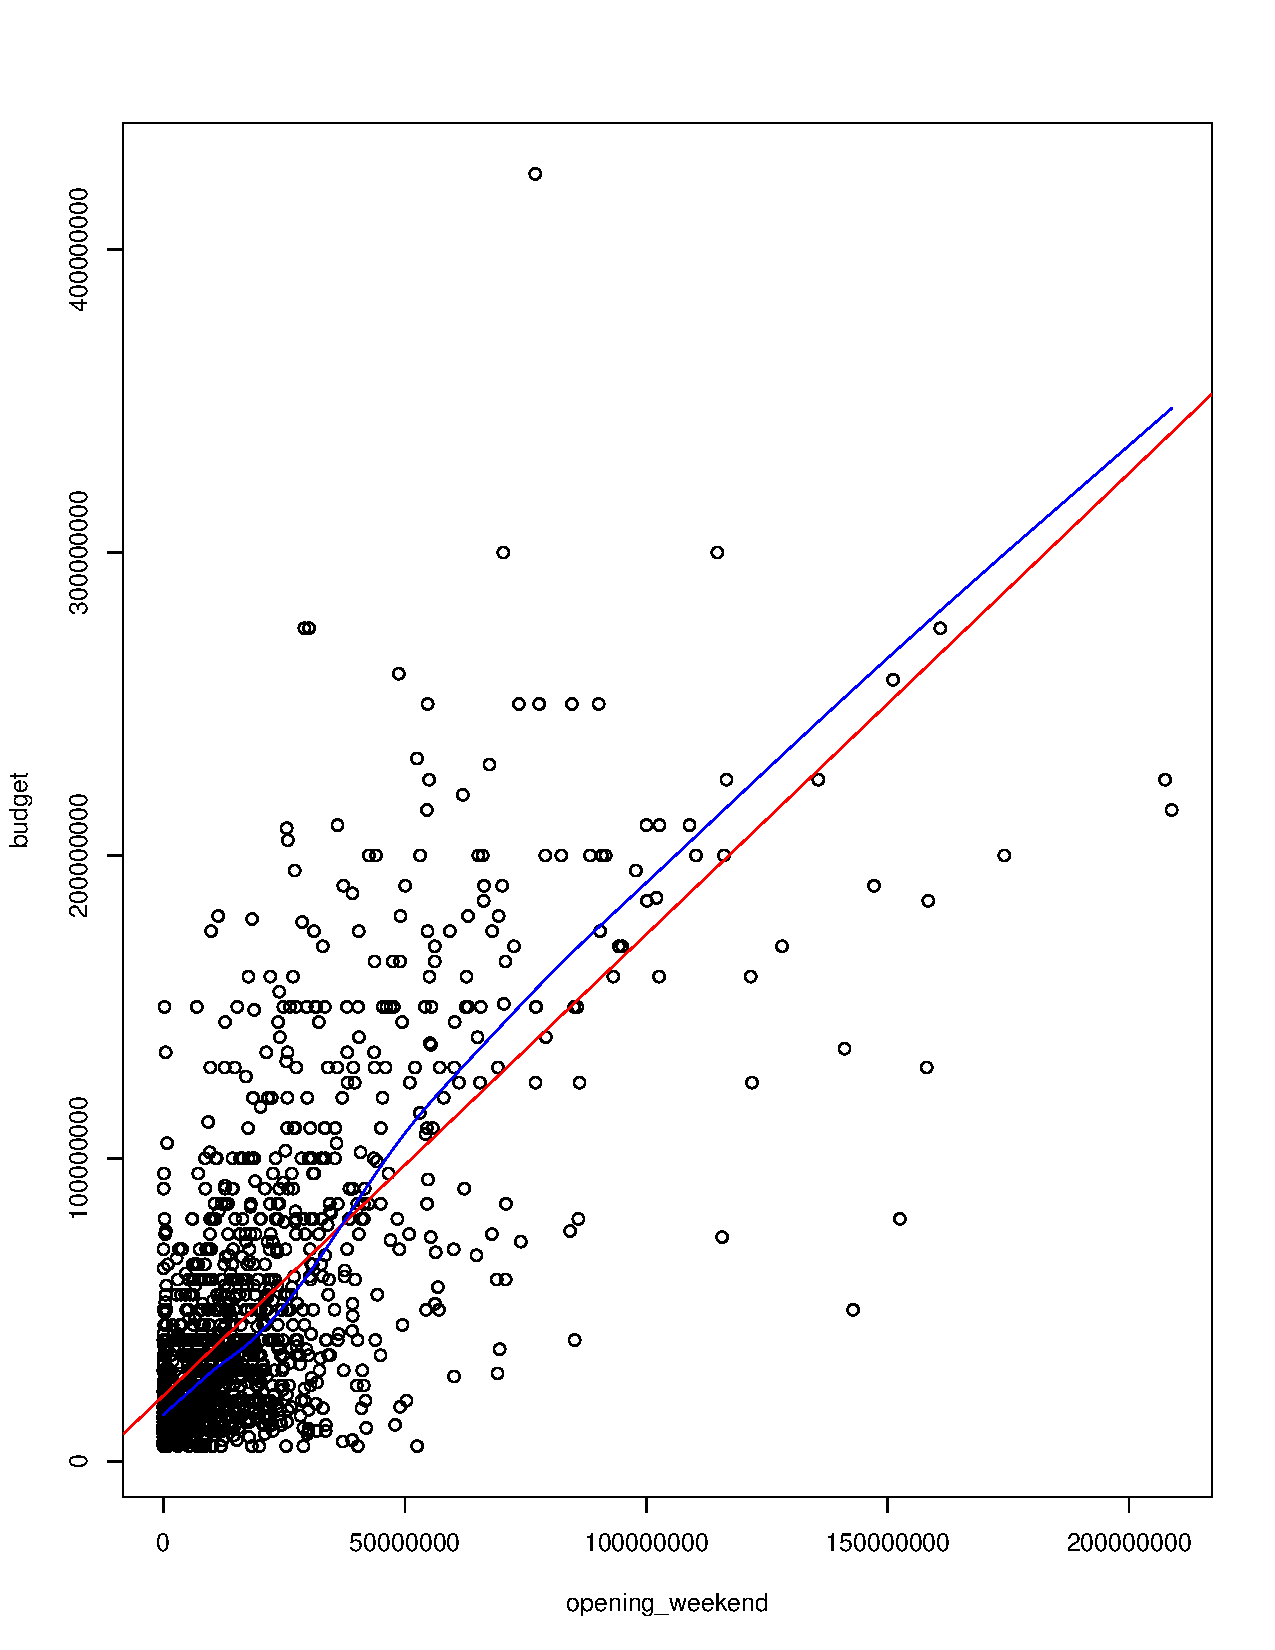
\includegraphics[scale=0.4]{LinearRegression1.pdf}

Linear Regressions make several underlying assumptions, most importantly that the residuals follow a gaussian (normal) distribution with zero mean and constant variation.  


\subsection{Logistic Regression}

Logistic Regression functions similarly to linear regression but provides binary output (fitting between 0 and 1).  Thus logistic regression is preferred for solving classification problems, while linear regressions are the method of choice for numerical problems.  

It is simple enough to perform a linear regression and compress the numeric output using a logit function $ \frac{1}{(1+e^{-t})} $.  Thus the logistic regression takes the form 
$$y = \frac{1}{1+e^{-(\theta_0+\theta_1x_2 + \theta_2x_2 + ...)}}$$.  

Here is some sample code

\vspace{3mm}

\begin{lstlisting}[language=R]

> formula <- isR ~ budget + opening_weekend + theaters + runtime
> 
> logisticModel <- glm(formula, data=traindata, family="binomial")
> 
> # Predict the probability for test data
> 
> prob <- predict(logisticModel, newdata=moviestest, type='response')
> round(prob, 3)
> cv.fit <- cv.glmnet(as.matrix(moviestrain[,c(-1,-2)]),
+                               as.vector(moviestrain[,3]),
+                               nlambda=100, alpha=0.7,
+                               family="gaussian")
> plot(cv.fit)
\end{lstlisting}

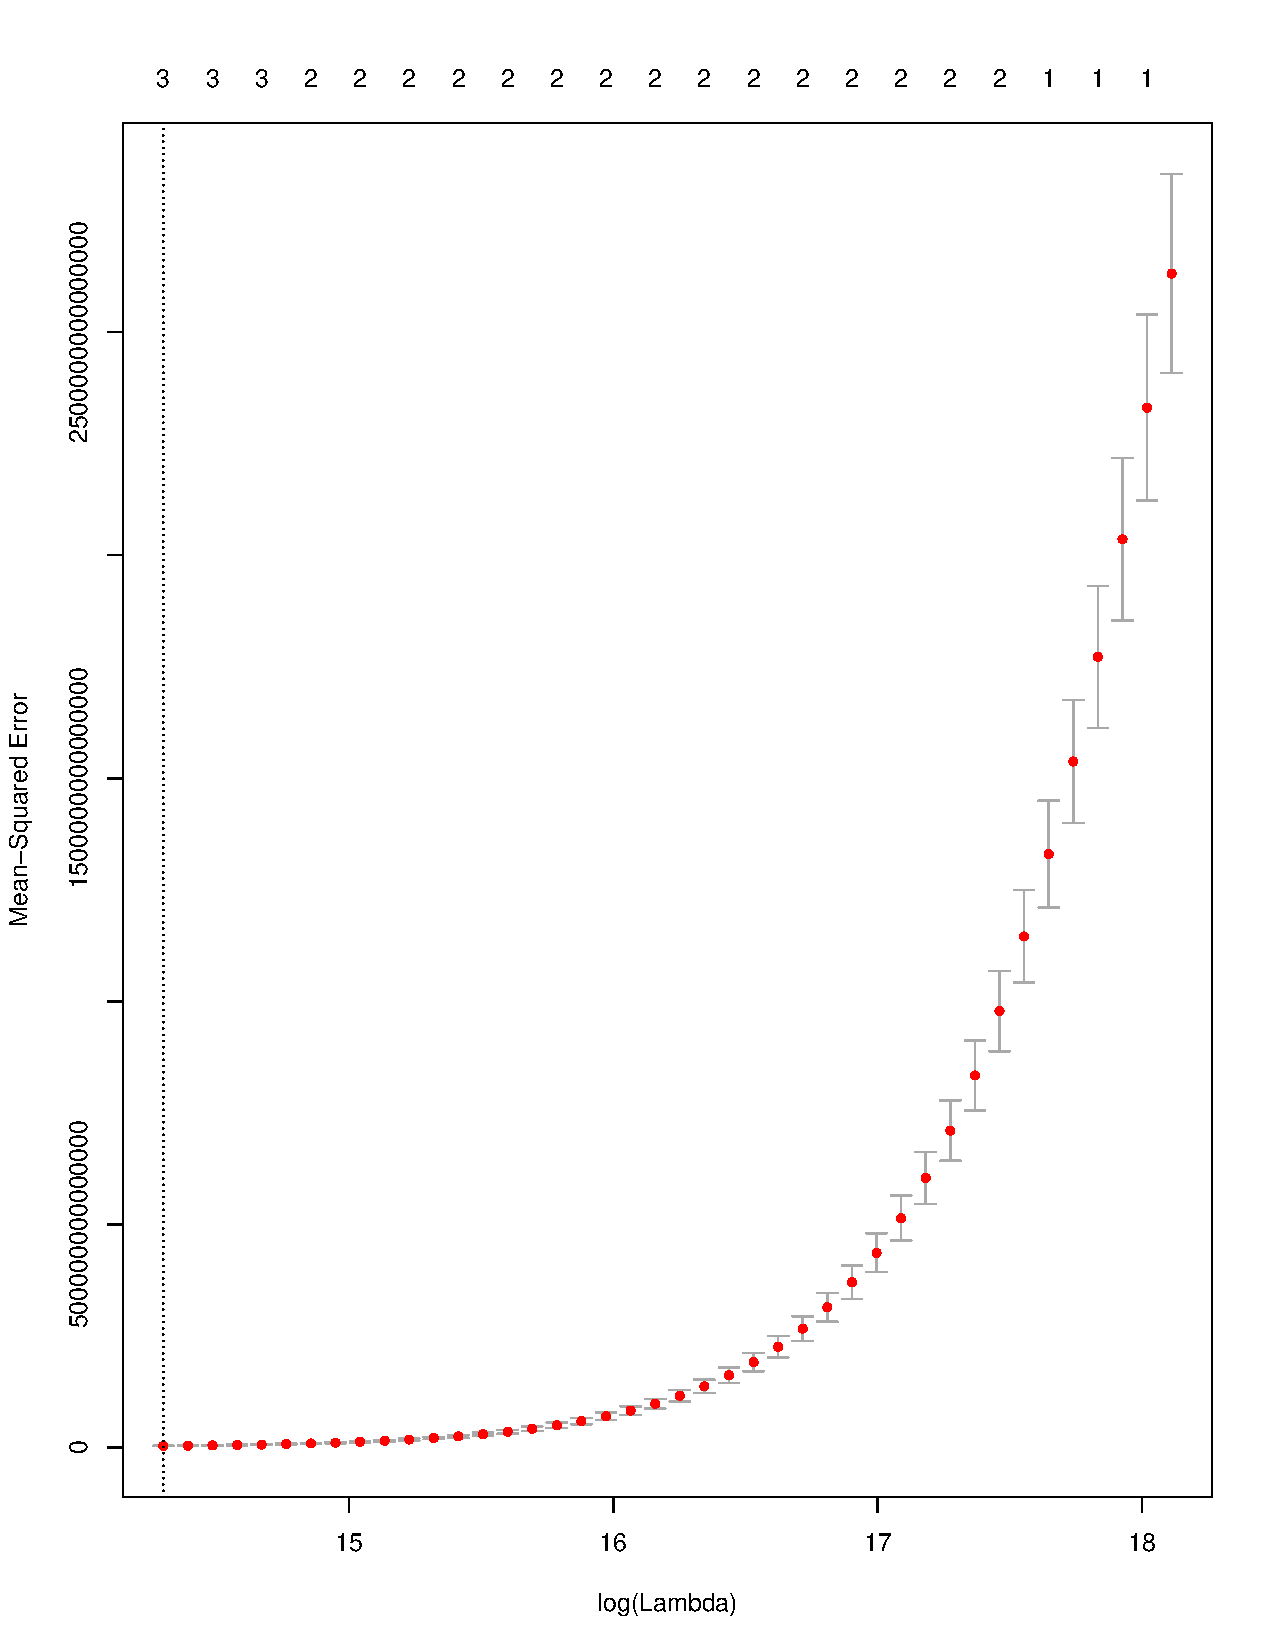
\includegraphics[scale=0.4]{logisticregression1.pdf}

\subsection{Regression with Regularization}

Linearity assumptions may often fail, making it necessary to combine existing features through multiplication.  With a large set of input variables but moderate size of training data, overfitting can often be an issue, causing the need for regularization to not fit too specifically.  

\vspace{3mm}

Overfitting occurs when $\theta$ has a large value, which we can correct by introducing a proportional penalty to it.  Ridge Regression and Lasso Regression are both ways of shrinking the magnitude of $\theta_i$, with Ridge Regression making dependent variables have uniform coefficients and Lasso Regression penalizing the coefficient of redundant variables linearly dependent.  The two methods of regression, also referred L1 and L2 regularization offers the function
$$ Cost = Nonregularization-cost + \lambda(\alpha.\sum||\theta_i|| + (1-\alpha).\sum \sqrt{\theta_i}) $$

In Ridge Regression the $\alpha$ parameter is tuned to 0, for Lasso Regression it's set to 1.  

\begin{lstlisting}[language=R]
> # Ridge Regression
> 
> # Fitting the ridge regression with alpha = 0 for ridge regression.
> grid = 10^seq(5, -2, length = 100)
> ridge.models = glmnet(x, y, alpha = 0, lambda = grid)
> #2 different coefficients, estimated 100 times --once each per lambda value.
> dim(coef(ridge.models))
[1]   3 100
> # Visualizing the ridge regression shrinkage.
> plot(ridge.models, xvar = "lambda", label = TRUE, main = "Ridge Regression")
> 
> # Creating training and testing sets. 70% of our data in the training, 30% in test
> set.seed(0)
> train = sample(1:nrow(x), 7*nrow(x)/10)
> test = (-train)
> y.test = y[test]
> 
> length(train)/nrow(x)
[1] 0.7
> length(y.test)/nrow(x)
[1] 0.3
> 
> # Performing cross-validation in order to choose the best lambda
> # 10-fold cross validation.
> set.seed(0)
> cv.ridge.out = cv.glmnet(x[train, ], y[train], lambda = grid, alpha = 0, nfolds = 10)
> plot(cv.ridge.out, main = "Ridge Regression\n")
> bestlambda.ridge = cv.ridge.out$lambda.min
> bestlambda.ridge
[1] 84975.34359
> log(bestlambda.ridge)
[1] 11.35011642
> 
> # MSE associated with this best value of lambda
> ridge.bestlambdatrain = predict(ridge.models, s = bestlambda.ridge, newx = x[test, ])
> mean((ridge.bestlambdatrain - y.test)^2)
[1] 249227604754637
> 
> # Refitting ridge regression on overall dataset using the best lambda value
> ridge.out = glmnet(x, y, alpha = 0)
> predict(ridge.out, type = "coefficients", s = bestlambda.ridge)
3 x 1 sparse Matrix of class "dgCMatrix"
                              1
(Intercept) -6305778.9959886819
budget             0.2245052367
theaters        6116.3988968179
> 
> # Inspection of MSE for our final ridge model
> ridge.bestlambda = predict(ridge.out, s = bestlambda.ridge, newx = x)
> mean((ridge.bestlambda - y)^2)
[1] 239905855805435
> 
> # Lasso Regression
> 
> #Fitting lasso regression with alpha = 1
> lasso.models = glmnet(x, y, alpha = 1, lambda = grid)
> 
> dim(coef(lasso.models))
[1]   3 100
> # Cross-validation to choose lambda
> # 10-fold cross validation.
> set.seed(0)
> cv.lasso.out = cv.glmnet(x[train, ], y[train], lambda = grid, alpha = 1, nfolds = 10)
> plot(cv.lasso.out, main = "Lasso Regression\n")
> bestlambda.lasso = cv.lasso.out$lambda.min
> bestlambda.lasso
[1] 0.01
> log(bestlambda.lasso)
[1] -4.605170186
> 
> # test MSE associated with this lambda?
> lasso.bestlambdatrain = predict(lasso.models, s = bestlambda.lasso, newx = x[test, ])
> mean((lasso.bestlambdatrain - y.test)^2)
[1] 249199216390375
> 
> #Refitting
> lasso.out = glmnet(x, y, alpha = 1)
> predict(lasso.out, type = "coefficients", s = bestlambda.lasso)
3 x 1 sparse Matrix of class "dgCMatrix"
                             1
(Intercept) -7097984.995270934
budget             0.237012655
theaters        6202.081428126
> 
> #Insepcting MSE
> lasso.bestlambda = predict(lasso.out, s = bestlambda.lasso, newx = x)
> mean((lasso.bestlambda - y)^2)
[1] 239208747378808
\end{lstlisting}

\section{Neural Networks}

Neural Networks involve a network of interconnected neurons sending signals to one another.  Each neuron in a neural network represents a logistic regression unit, and the neurons are organized in multiple layers where every neuron connects to the neurons at the next level.  

\begin{lstlisting}[language=R]
> # Neural Networks
> 
> nnet_moviestrain <- moviestrain
> #Binarize the categorical output
> nnet_moviestrain <- cbind(nnet_moviestrain, moviestrain$mpaa_rating == 'R')
> nnet_moviestrain <- cbind(nnet_moviestrain, moviestrain$mpaa_rating == 'PG-13')
> nnet_moviestrain <- cbind(nnet_moviestrain, moviestrain$mpaa_rating == 'NOT RATED')
> names(nnet_moviestrain)[6] <- 'R'
> names(nnet_moviestrain)[7] <- 'PG_13'
> names(nnet_moviestrain)[8] <- 'NOT_RATED'
> nn <- neuralnet(R + PG_13 + NOT_RATED ~ budget + opening_weekend, data=nnet_moviestrain, hidden=c(3))
\end{lstlisting}

\vspace{3mm}

The neural network includes hidden layers, number of neurons and learning rate.  Since there are no fixed rules for neural networks, they are a fairly versatile tool specifically thanks to iterative feedback mechanisms.  

\vspace{3mm}

Furthermore, neural networks are often successful at learning non-linear functions and multiple outputs, especially when multiple rounds are conducted.  

\section{Support Vector Machines}

Support Vector Machines are applied on data that is linearly seperable and function by finding a dividing hyperplane between a set of samples.  The problem can typically be framed as a quadratic programming optimization problem, as data output on one side must balance with that on the other.  In the case that data is not linearly seperable due to noise, an error term can be added to penalize the optimization.  

\vspace{3mm}

If the data is fundamentally non-linear, a data transformation must be performed and the data must be moved to a higher dimension.  The optimization term becomes a dot product of the transformed points which in the higher dimensional space which is equivalent to the kernelfunction results in the original space.  

\vspace{3mm}

Kernel functions offer a solution to performing quadratic optimization in higher dimensional spaces.  The tuning parameters include the penalty and cost variables, so the usual way of training an SVM model involves first finding the optimal parameters and then training the model.  

\begin{lstlisting}[language=R]
> #tune <- tune.svm(mpaa_rating~ opening_weekend + budget + theaters + runtime,
> #                 data=moviestrain,
> #                 gamma=10^(-6:1),
> #                 cost=10^(1:4))
> #summary(tune)
> 
> #model <- svm(mpaa_rating~ opening_weekend + budget + theaters + runtime,
> #             data = moviestrain,
> #             method="C=classification",
> #             kernel = "radial",
> #             probability=T,
> #             gamma=0.001,
> #             cost=1000)
> #prediction <- predict(model, moviestest)
> #table(moviestest$mpaa_rating, prediction)
\end{lstlisting}

Support vector machines with kernel functions is found to be extremely effective and extensible.  Despite being a binary classifier it can ben extended to multi-class classification by training a group of binary classifiers.  

\vspace{3mm}

SVM predicts output based on the distance to the dividing hyperplane which doesn't directly provide a probability estimation, but calibration techniques can be performed to learn a logistic regression model between the hyperplane and the binary output, allowing for a logistic regression to estimate probabilities.  

\vspace{3mm}

In non-linear classification problems SVM is extremely popular, particular when the set of input features is small as it allows for expansion into higher dimension space, assuming proper training data.  SVM is a more computationally intense method though, particularly with large training sets, so at times logistic regression with manually expanded feature sets can be more practical.  

\section{N{\"a}ive Bayes}

N{\"a}ive Bayes assumes that each input variable is independent of each other given output.  Thus, each input term can be learned by counting the training data.  When the inputs are numeric, we can assume normality which allows us to estimate probabilities.  

\vspace{3mm}

The main strength of N{\"a}ive Bayes is that it is highly scalable and learns incrementally since the only measure is observed variables.  Thus the model can perform well even in the absence of true independence.  

\begin{lstlisting}[language = R]
> # Naive Bayes
> # Handles both categorical and numeric input, but generally categorical is preferred
> model <- naiveBayes(mpaa_rating ~ opening_weekend + budget + theaters + runtime, data=moviestrain)
> prediction <- predict(model, moviestest[,-5])
> table(prediction, moviestest[,5])
\end{lstlisting}


\section{K Nearest Neighbor}

The K Nearest Neighbor technique contrasts with model-based learning and works by memorizing all training data.  To make predictions we find the closest K neighbors from the training set and allow them to vote for a final prediction.  

\vspace{3mm}

To determine said 'nearest neighbors' a distance function is defined.  Additionally, the voting can be weighted based on distance.  

\vspace{3mm}

K Nearest Neighbor techniques are advantageous due to their simplicity, as the incremental learning occurs automatically as more data arrives.  However, it stalls in higher dimensions and is quite computationally intense.  

\vspace{3mm}

\begin{lstlisting}[language=R]

> # K Nearest Neighbor
> 
> train_input <- as.matrix(moviestrain[,-5])
> train_output <- as.vector(moviestrain[,5])
> test_input <- as.matrix(moviestest[,-5])
> prediction <- knn(train+input, test_input, train_output, k=5)

\end{lstlisting}

\section{Decision Trees}

Decision trees are based on a set of decision nodes which decide recursively how to discriminatively divide training data into buckets of homogenous members.  For categorical data this homogeneity is based on output label - for numeric values it is variance and for categorical it is the gini index.  

\vspace{3mm}

During training various dividing criteria are tried until there is no significant gain in homogeneity by further splits.  The members of the bucket represented at leaf node will vote for the prediction and the majority wins for categorical output and average is taken for numerical output.  

\vspace{3mm}

\begin{lstlisting}[language=R]
> # Decision Tree
> 
> # Training the decision tree
> treemodel <- rpart(mpaa_rating ~ opening_weekend + budget + theaters, data=moviestrain)
> plot(treemodel)
> text(treemodel, use.n=T)
> # Predict using decision tree
> prediction <- predict(treemodel, newdata=moviestest, type='class')
> # Contingency table determines accuracy
> table(prediction, moviestest$mpaa_rating)
           
prediction    G NC-17 NOT RATED  PG PG-13   R UNRATED
  G           0     0         0   0     0   0       0
  NC-17       0     0         0   0     0   0       0
  NOT RATED   0     0         0   0     0   0       0
  PG          0     0         0   0     0   0       0
  PG-13       3     0         0  57   130  73       0
  R           2     0         3   4    27  66       0
  UNRATED     0     0         0   0     0   0       0
\end{lstlisting}

\vspace{3mm}

The advantage of a tree is that it can take different sorts of input and output variables which can be categorical, binary or numerical.  It also handles outlieres well and explains it's prediction reasoning fairly effectively.  

\vspace{3mm}

The main constraint of decision trees is the binary nature of the decisions.  Furthermore, decision criteria only consider one input attributes at a time, not a combination of multiple input variables.  Finally, once it's learned it cannot be updated incrementally.  

\section{Tree Ensembles}

Ensemble Methods combine multiple models to fit the data, through both either bagging or boosting.  

\vspace{3mm}

In bagging a subset of the trained data is taken (usually random sample with replacement) to train each model.  After several models have been trained a voting scheme predicts future data.  

\vspace{3mm}

In boosting the training data records are sampled with an increased emphasis on wrongly predicted data.  Initially each training data is uniformly weighted but at each iteration data that is wrongly classified undergoes an increase in it's weight.  The final prediction is voted by each tree at each iteration.  


\subsection{Random Forests}

Random Forests are a popular bagging model which work by selecting n training data out of N, at each decision node.  It also randomly selects m input features from the total M input features and learns a decision tree from it.  

\vspace{3mm}

\begin{lstlisting}[language=R]
> # Random Forest
> 
> # Trains 100 trees with randomly selected attributes
> model <- randomForest(mpaa_rating ~ opening_weekend + budget + theaters, data=moviestrain, nTree=500)
> # Predict using the forest
> prediction <- predict(model, newdata=moviestest, type='class')
> table(prediction, moviestest$mpaa_rating)
           
prediction   G NC-17 NOT RATED PG PG-13  R UNRATED
  G          0     0         0  0     1  0       0
  NC-17      0     0         0  0     0  0       0
  NOT RATED  0     0         0  0     0  0       0
  PG         2     0         0 18    11  8       0
  PG-13      1     0         1 33    86 38       0
  R          2     0         2 10    59 93       0
  UNRATED    0     0         0  0     0  0       0
> importance(model)
                MeanDecreaseGini
opening_weekend      244.5383998
budget               186.5633371
theaters             233.5496660
\end{lstlisting}

\subsection{Gradient Boosted Trees}

In gradient boosted trees, a popular boosting method, functions are incrementally added that fit with the gradient of a lost function of residuals.  

\vspace{3mm}

\begin{lstlisting}[language=R]
> # Gradient Boosted Trees
> 
> movies2 <- movies
> newcol = data.frame(isR=(movies2$mpaa_rating=='R'))
> movies2 <- cbind(movies2, newcol)
> movies2[45:55,]
                   title mpaa_rating   budget
45              Firewall       PG-13 50000000
46        Curious George           G 50000000
47   Final Destination 3           R 25000000
48        The Shaggy Dog          PG 60000000
49     Failure to Launch       PG-13 50000000
50   The Hills Have Eyes           R 17000000
51                 Babel           R 20000000
52           A Good Year       PG-13 35000000
53 Stranger Than Fiction       PG-13 30000000
54                  Zoom          PG 35000000
55                 Pulse       PG-13 20500000
   log_budget opening_weekend runtime theaters year
45       7.70        13635463     105     2840 2006
46       7.70        14703405      86     2566 2006
47       7.40        19173094      93     2880 2006
48       7.78        16310058      98     3501 2006
49       7.70        24411322      97     3057 2006
50       7.23        15708512     107     2620 2006
51       7.30          389351     143        7 2006
52       7.54         3721526     117     2066 2006
53       7.48        13411093     113     2264 2006
54       7.54         4510408      83     2501 2006
55       7.31         8203822      90     2323 2006
     isR
45 FALSE
46 FALSE
47  TRUE
48 FALSE
49 FALSE
50  TRUE
51  TRUE
52 FALSE
53 FALSE
54 FALSE
55 FALSE
> 
> formula <- isR ~ opening_weekend + budget + theaters
> model <- gbm(formula, data=movies2,
+              n.trees=1000,
+              interaction.depth=2,
+              distribution="bernoulli")
> prediction <- predict.gbm(model, movies2[45:55,],
+                           type="response",
+                           n.trees=1000)
> round(prediction, 3)
 [1] 0.416 0.417 0.419 0.191 0.412 0.419 0.553 0.421
 [9] 0.418 0.421 0.420
> summary(model)
                            var      rel.inf
theaters               theaters 77.426620680
opening_weekend opening_weekend 13.916420039
budget                   budget  8.656959281
\end{lstlisting}

\section{Evaluation of Model Performance}

Any evaluation of a model ought to be held against a random guess for categorical data or a mean of output of training samples for numerical data at a minimum.  Beyond that it's valuable to set a precise goal - whether it be the best model at the moment or the expected best model over time.  

\vspace{3mm}

Typically data is divided into three disjoint groups - 20 percent being set aside as testing data, 80 percent divided into k partitions where k-1 consist of training data and 1 partition used as a cross-validation to choose optimal parameter values.  

\vspace{3mm}

Regression performance can be measured by measuring the distance between estimated output and actual output, or measuring the sum of square error.  The three measures typically observed are root mean square error, relative square error and coefficient of determination.  

\vspace{2mm}

Mean Square Error (MSE) = $\frac{1}{N} * \sum (y_{est} - y_{actual})^2$

Root Mean Square Error (RMSE) = $(MSE)^{\frac{1}{2}}$

Relative Square Error RSE = $\frac{MSE}{MSE_{baseline}}$ = $\frac{\sum(y_{est} - y_{actual})^2}{(y_{mean}-y_{actual})^2}$

$R^2 = 1 - RSE = \frac{(MSE_{baseline} - MSE)}{MSE_{baseline}}$

\vspace{3mm}

\begin{lstlisting}[language=R]
> # Measuring Regression Performance
> 
> # -----------------------------------------------------------------------------------------------
> # debug
> movies_clean <- movies[!is.na(movies$mpaa_rating),]
> model <- lm(opening_weekend~ budget + theaters, data=movies_clean)
> score <- predict(model, newdata=movies_clean)
> actual <- movies_clean$movies
> rmse <- (mean((score - actual)^2))^0.5
> rmse
[1] NaN
> mu <- mean(actual)
Warning message:
In mean.default(actual) : argument is not numeric or logical: returning NA
> rse <- mean((score-actual)^2 / mean(mu-actual)^2)
> rse
[1] NaN
> rsquare <- 1 - rse
> rsquare
[1] NaN
\end{lstlisting}

MSE penalizes the bigger difference exponentially due to the square effect - to reduce this we can simply take the log transform.  

vspace{3mm}

Mean Square Log Error MSLE = $(\frac{1}{N}*\sum(log(y)_est-log(y)_{actual})^2$

Root Mean Square Log Error RMSLE = $(MSLE)^{\frac{1}{2}}$

\vspace{3mm}

Both bias and variance provide potential sources of error.  Bias issues occur when an unfit model is used to represent the underlying data, and results in both training and cross-validation having high error rates, both dropping as model complexity increases.  Variation problems occur when model parameters fit too specifically to the training data but not well to the underlying data pattern.  Variance issues emerge when there is insufficient training data to compare to the number of model parameters.  

\vspace{3mm}

To evaluate whether more data ought to be obtained one can plot the error against the size of data.  Thus one can plot both cross-validation error and training error with respect to training sample size.  

\vspace{3mm}

In situations featuring high-bias, efforts should be put towards adding more input features by either identifying more input signals or combining existing input features in non-linear ways.  Additionally, one can increase the complexity of the model.  

\vspace{3mm}

In high variance problems where model complexity is over-estimated, a reduction in model complexity can improve the performance of the model.  

\section{Conclusion}

Since robust data can be tricky to come across in the film prediction sphere it's worthwhile to consider models where the complexity can readily be adapted.  Thus, my advisor and I have determined a focus on neural networks will be best moving forward.  Ideally in any analytic space a variety of learning methods ought to be applied, favoring ensemble learning techniques such as bagging and boosting.  Further exploration into stacking is needed though before any implementation can be recommended.  At the moment we will move on to studying neural networks and deep learning with increased specificity.  


\end{spacing}

\end{document}
